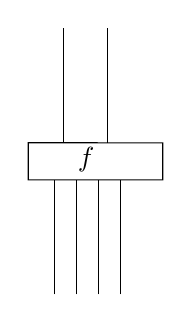
\begin{tikzpicture}[yscale=-1,scale=0.02,baseline={([yshift=-.5ex]current bounding box.center)}]
\begin{scope}[shift={(0.00mm,719.29mm)}]
% path id='path3336'
% path spec='m 432.44069,30.59292 0,235.46656 854.18501,0 0,-234.75945 z'
\draw [fill=none,draw=black] (432.44mm,30.59mm)
-- ++(0.00mm,235.47mm)
-- ++(854.19mm,0.00mm)
-- ++(0.00mm,-234.76mm)
-- cycle
;
% path id='path3338'
% path spec='m 656.19509,30.471607 0,-726.905767'
\draw [fill=none,draw=black] (656.20mm,30.47mm)
-- ++(0.00mm,-726.91mm)
;
% path id='path3340'
% path spec='m 936.19509,30.471607 0,-726.905767'
\draw [fill=none,draw=black] (936.20mm,30.47mm)
-- ++(0.00mm,-726.91mm)
;
% path id='path3342'
% path spec='m 598.19509,992.4716 0,-726.90578'
\draw [fill=none,draw=black] (598.20mm,992.47mm)
-- ++(0.00mm,-726.91mm)
;
% path id='path3344'
% path spec='m 878.19509,992.4716 0,-726.90578'
\draw [fill=none,draw=black] (878.20mm,992.47mm)
-- ++(0.00mm,-726.91mm)
;
% path id='path3346'
% path spec='m 736.19509,992.4716 0,-726.90578'
\draw [fill=none,draw=black] (736.20mm,992.47mm)
-- ++(0.00mm,-726.91mm)
;
% path id='path3348'
% path spec='m 1016.1951,992.4716 0,-726.90578'
\draw [fill=none,draw=black] (1016.20mm,992.47mm)
-- ++(0.00mm,-726.91mm)
;
\node [black] at (800.00mm,140.36mm) { $f$ };
\end{scope}
\end{tikzpicture}
